\documentclass{article}
\usepackage[backend=biber,natbib=true,style=authoryear,maxbibnames=10]{biblatex}
\addbibresource{/home/nqbh/reference/bib.bib}
\usepackage[utf8]{vietnam}
\usepackage{tocloft}
\renewcommand{\cftsecleader}{\cftdotfill{\cftdotsep}}
\usepackage[colorlinks=true,linkcolor=blue,urlcolor=red,citecolor=magenta]{hyperref}
\usepackage{amsmath,amssymb,amsthm,float,graphicx,mathtools,tikz}
\usetikzlibrary{calc,angles}
\allowdisplaybreaks
\newtheorem{assumption}{Assumption}
\newtheorem{baitoan}{Bài toán}
\newtheorem{cauhoi}{Câu hỏi}
\newtheorem{conjecture}{Conjecture}
\newtheorem{corollary}{Corollary}
\newtheorem{dangtoan}{Dạng toán}
\newtheorem{definition}{Definition}
\newtheorem{dinhly}{Định lý}
\newtheorem{dinhnghia}{Định nghĩa}
\newtheorem{example}{Example}
\newtheorem{ghichu}{Ghi chú}
\newtheorem{hequa}{Hệ quả}
\newtheorem{hypothesis}{Hypothesis}
\newtheorem{lemma}{Lemma}
\newtheorem{luuy}{Lưu ý}
\newtheorem{nhanxet}{Nhận xét}
\newtheorem{notation}{Notation}
\newtheorem{note}{Note}
\newtheorem{principle}{Principle}
\newtheorem{problem}{Problem}
\newtheorem{proposition}{Proposition}
\newtheorem{question}{Question}
\newtheorem{remark}{Remark}
\newtheorem{theorem}{Theorem}
\newtheorem{vidu}{Ví dụ}
\usepackage[left=1cm,right=1cm,top=5mm,bottom=5mm,footskip=4mm]{geometry}
\def\labelitemii{$\circ$}
\DeclareRobustCommand{\divby}{%
	\mathrel{\vbox{\baselineskip.65ex\lineskiplimit0pt\hbox{.}\hbox{.}\hbox{.}}}%
}

\title{TikZ}
\author{Nguyễn Quản Bá Hồng\footnote{Independent Researcher, Ben Tre City, Vietnam\\e-mail: \texttt{nguyenquanbahong@gmail.com}; website: \url{https://nqbh.github.io}.}}
\date{\today}

\begin{document}
\maketitle
\begin{abstract}
	A personal practice of drawing figures in \LaTeX\ by using TikZ package.
\end{abstract}
\tableofcontents
\newpage

%------------------------------------------------------------------------------%

\section{Hệ Trục Tọa Độ}
See \cite[p. 9]{Quy2022}.

\begin{tikzpicture}[>=stealth,scale=.75]
	\draw[->](-3,0)--(3,0) node[above]{$x$};
	\draw[->](0,-3)--(0,3) node[left]{$y$};
	\draw[dashed](0,1)--(2,1)--(2,0);
	\draw(2,1) circle(0.05) node[above right]{$A$};
	\path(0,0) node [below left]{$O$};
\end{tikzpicture}
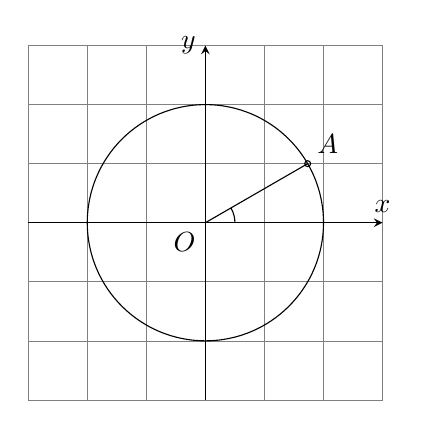
\begin{tikzpicture}[>=stealth,scale=.75]
	\draw[step=1,gray,very thin](-3,-3) grid (3,3);
	\draw[->](180:3)--(0:3) node[above]{$x$};
	\draw[->](-90:3)--(90:3) node[left]{$y$};
	\draw(0,0) circle(2);
	\draw(0,0)--(30:2) (0:.5) arc(0:30:.5);
	\draw(30:2) circle(0.05) node[above right]{$A$};
	\path(0:0) node[below left]{$O$};
\end{tikzpicture}

\begin{tikzpicture}
	\draw[step=1,gray,very thin](-2,-1) grid (3,2);
\end{tikzpicture}
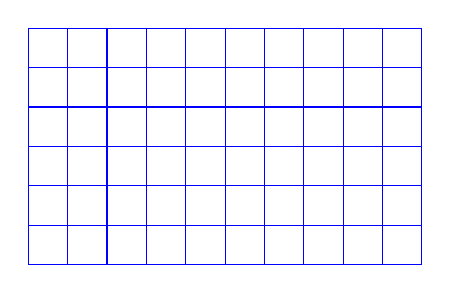
\begin{tikzpicture}
	\draw[step=.5,blue,thin](-2,-1) grid (3,2);
\end{tikzpicture}
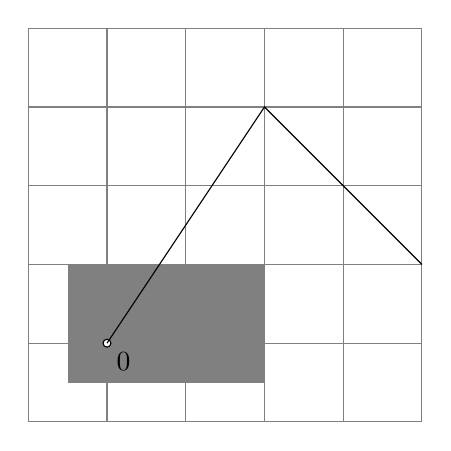
\begin{tikzpicture}
	\draw[step=1,gray,thin](-1,-1) grid (4,4);
	\fill[gray](-.5,-.5) rectangle (2,1);
	\draw[fill=white] (0:0) circle (.05);
	\draw(0:0)--(2,3)--(4,1);
	\path(0:0) node[below right]{$0$};
\end{tikzpicture}
\begin{tikzpicture}[declare function={c=sqrt(3);}]
	\coordinate[label=above:A](A) at (1,2);
	\coordinate (A) at (30:2);
	\path
	(1,2) coordinate[label=above:A] (A)
	(2,5) coordinate[label=right:B] (B)
	(4,2) coordinate[label=left:C] (C);
	\def\a{3}
	\pgfmathsetmacro\b{2*sqrt(2)}
	\draw (0:0) circle (\a);
	\draw (0:0) circle (c);
%	\path
%	\coordinate (H) at ($(A)+(B)$);
%	\coordinate[label=above:D] (D) at ($(A)!.5!(B)$);
%	\coordinate (E) at ($(A)!1!30:(B)$);
%	\coordinate (F) at ($(A)!.5!30:(B)$);
%	\coordinate (G) at (intersection of A--B and C--D);
\end{tikzpicture}
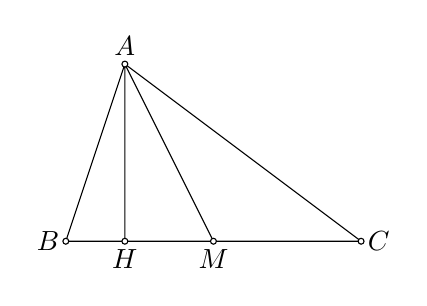
\begin{tikzpicture}[scale=.75]
	\path
	(1,3) coordinate (A)
	(0,0) coordinate (B)
	(5,0) coordinate (C)
	($(B)!(A)!(C)$) coordinate (H)
	($(B)!.5!(C)$) coordinate (M);
	\draw (A)--(B)--(C)--cycle (A)--(H) (A)--(M);
	\foreach \x/\g in {A/90,B/180,C/0,H/-90,M/-90} \draw[fill=white] (\x) circle (.05) + (\g:.3) node{$\x$};
\end{tikzpicture}

%------------------------------------------------------------------------------%

\section{Vẽ Điểm}

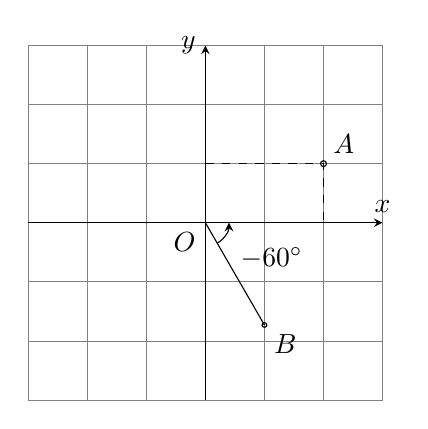
\begin{tikzpicture}[>=stealth,scale=.75]
	\draw[step=1,gray,very thin](-3,-3) grid (3,3);
	\draw[->](-3,0)--(3,0);
	\draw[->](0,-3)--(0,3);
	\draw[dashed](0,1)--(2,1)--(2,0);
	\draw(2,1) circle(.05);
	\draw(3,0) node[above]{$x$} (0,3) node[left]{$y$} (0,0) node[below left]{$O$};
	\draw(-60:2) circle(0.04);
	\draw(-60:2) -- (0,0);
	\draw(2,1) node[above right]{$A$} (-60:2) node[below right]{$B$};
	\draw[->](-60:4mm) arc(-60:0:4mm);
	\path(-30:5mm) node[below right]{$-60^\circ$};
\end{tikzpicture}

%------------------------------------------------------------------------------%

\printbibliography[heading=bibintoc]
	
\end{document}